\documentclass[letter paper, 12pt]{article}
\usepackage[english]{babel}
\usepackage{amsmath}
\usepackage{amsfonts}
\usepackage{amssymb}
\usepackage{gensymb}
\usepackage{changepage}
\usepackage[margin=1in]{geometry}
\usepackage{epsfig}
\usepackage{enumerate}
\usepackage{mathtools}
\usepackage{wasysym}
\usepackage[normalem]{ulem}

\usepackage{tikz-er2}
\newcommand{\ra}{\rightarrow}
\newcommand{\tab}{${}_{}$\hspace{0.2in}}
\newcommand{\noin}{\noindent}


\begin{document}
\noindent Finn Lidbetter and Micah Stairs\\
Comp 3721\\
Dr. Ricker\\
\today \bigskip
\begin{center}
	{\Large Shopping Penguin Design Document}
\end{center}
\underline{Design Decisions}\vspace{5pt}

\noin \tab In order to help realise Shopping Penguin's dream, we designed the structure for an e-commerce site that would allow a user to order fish-flavoured lollipops and musical slippers. This structure was designed with Object Oriented design principles in mind. The basic functionalities that we wanted to implement were:
\begin{itemize}
	\item The ability to fill a shopping cart with items in the store
	\item The ability to empty this shopping cart
	\item Handling of shipping information
	\item Handling of various popular payment methods
	\item Processing an order
	\item Producing objects according to an order
\end{itemize}
With these functionalities in mind, we designed a solution that incorporates several design patterns and pays particular attention to the Single Responsibility Principle. \\
\tab We decided to use a Decorator pattern for our shopping cart. The idea behind this is that a user would decorate an empty shopping cart with the items that they wish to purchase. By using a decorator pattern we are able to aggregate the cost of all of the items in the cart and maintain a list of the items through a single reference to an object that is initially an empty cart. The concrete components of this decorator pattern, with which the shopping cart can be decorated, are defined in the Item enum type. This allows for a simple means to introduce new items that could be added to the shopping cart if necessary. In the current implementation, the only items that can be added to the shopping cart are the 3 fish-flavoured lollipops and the 2 pairs of musical slippers.\\
\tab We wanted our design to only construct the Lollipop and Slipper objects once the order was placed. Furthermore, we didn't want to require that the part of the structure responsible for placing orders must know how to build the Lollipop and Slipper objects. To satisfy these desires we made use of 2 factory classes and an abstract factory class. The abstract factory defines the common behaviour of the Lollipop and Slipper factories, and then these 2 concrete factory classes handle the creation of Lollipop and Slipper objects according to the orders that are placed.\\
\tab Finally, we wanted to allow orders to be processed using a variety of different payment methods. We provided functionality for 3 different debit-based payment methods (gift card, PayPal, and Bitcoin) and 1 credit based method (credit card). These payment methods were separated out according to the differences and similarities between them. In particular, they are all payment methods through which money can be charged. However, the way in which the accounts/cards are charged differs depending on whether they are credit or debit based. This is reflected in our design.\\
\tab Overall, our code is designed to meet Shopping Penguin's requirements while adhering to Object Oriented design principles. We believe that we have achieved this through our choice of design patterns, and the structure of the relationships and dependencies in our design.
\vspace{1in}

\begin{figure}[h]
	\caption{Classes and enum involved in the Factories in our design}
	\includegraphics[scale=0.9]{FactoryUML}
\end{figure}
\newpage

\begin{figure}[h]
	\caption{Classes, interface, and enum involved in the Decorator in our design}
	\noin\includegraphics{DecoratorUML}
\end{figure}
\newpage
\begin{figure}[h]
	\caption{Classes and interface involved in the Payment Method part of our design}
	\noin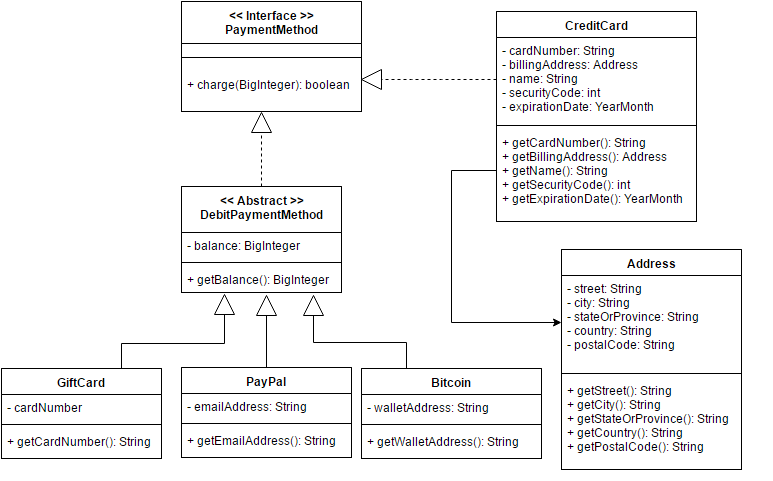
\includegraphics[scale=0.9]{PaymentUML}
\end{figure}
\end{document}